\documentclass[10pt]{article}
\usepackage[utf8]{inputenc}
\usepackage[T1]{fontenc}
\usepackage{mathtools} % Charge amsmath.
\usepackage{amssymb}
\usepackage{circuitikz}
\usepackage{fontspec}
\usepackage{array}
\usepackage{float}

\setmainfont{Times New Roman}

%
% NOTE: schematics generated using the online tool: 'https://www.circuit2tikz.tf.fau.de/designer'
%

\title{Vector Electronics}
\author{QuBi}
\date{\today}

\begin{document}

\maketitle

The purpose of this article is to describe an attempt to solve electronic circuits made of non-linear devices like diodes, bipolar transistors, JFETs, MOSFETs, etc. using linearisation techniques.\\

A common approach is to set the circuit at some operating point and wiggle it around with the input signal.
For small variations, even the most non-linear device can be approximated by a linear model.
The \textit{Small Signal Analysis}, as it is called, is a classical framework for that.\\

However, some circuits are trickier and make one or more non-linear devices operate way beyond the small signal hypothesis.

The class AB (push/pull) amplifier is one example: a transistor in the pair goes from cut-off to linear region as the input rises. 
The other transistor does the opposite. Meanwhile, the output follows the input nicely (the circuit as a whole surprisingly acts as if everything were linear.)\\

To fully analyse this, one could try to use a full model of the transistor (exponential curve) however:
\begin{itemize}
	\item the equations usually have no closed-form expression (equations combining $\exp()$ and polynomials) 
	\item it doesn't give much insight on \textit{how} the thing works.
\end{itemize}

\section*{The Piecewise Linear Model}
A non-linear continuous function can always be approximated by a piecewise affine (linear) function\footnote{In other words, the set of piecewise linear functions is dense in the space of continuous real-valued functions}, 
provided the model is refined and enough control points are introduced.
Thus, when analyzing a circuit, one can quite reasonably assume, as a first approximation, that the characteristic of a non-linear component is in fact piecewise linear. \\
The parameters of the linear relationship (slope and offset) may not yet be known for the present operating point, but they must necessarily correspond to one of the (slope, offset) pairs among those defined in the proposed piecewise affine model.\\

The task then reduces to determining which pair applies at a given operating point.
The existence of such a pair is "reassured" by the fact that every circuit necessarily has \textit{at least} one operating point. 
It is reasonable to assume that this solution is unique.\footnote{Even though certain "pathological" circuits (e.g. with feedback) may admit multiple possible operating points (stable or not). We will return to this point later.}

For most practical cases, the overall result is that every component can be treated as linear, thereby enabling the full use of linear analysis techniques (superposition principle, etc.) without any loss of generality.\\

Notice that, since any linear transformation to a piecewise linear function is still a piecewise linear function, the very concrete consequence is that the piecewise-affine property of a non-linear component \textbf{propagates} to all the properties of the electronic circuit in which it is embedded.

In this sense, we speak in this paper of a \textit{Vector Analysis} of the circuit. If one views a piecewise-affine function as an element of a vector space (which it is) then the circuit's properties—whatever they may be: $V_{OUT}$ vs $V_{IN}$, $I/V$ characteristic, transmittance, input impedance, etc.—are likewise contained within that same vector space.\\

It may therefore be conceivable to interpret the action of a circuit on a nonlinear component as analogous to a matrix acting on a vector. The idea that a circuit might have a kind of “matrix analogue” is perhaps worth exploring further.


\section*{Example 1: Diode and Resistor I}
In most lectures about semiconductors, one of the first case study is the resistor-diode circuit. It corresponds to most of the LED polarisation circuits.

\begin{circuitikz}
	\node[eground2] at (2, 1){};
	\draw (2, 2.5) to[empty diode, l={$D$}] (2, 1);
	\draw (2, 4.5) to[american resistor, /tikz/circuitikz/bipoles/length=1.05cm, l={$R$}] (2, 2.5);
	\draw (2, 4.5) |- (1, 5);
	\node[ocirc](N1) at (1, 5){} node[anchor=east] at (N1.west){$V$};
	\draw[line width=1.6pt, -latex] (3.5, 1.25) -- (3.5, 2.5);
	\draw[dash pattern={on 0.4pt off 1.6pt}] (2.25, 2.75) -- (3.5, 2.75);
	\draw[dash pattern={on 0.4pt off 1.6pt}] (2.25, 1) -- (3.5, 1);
	\node[shape=rectangle, minimum width=0.715cm, minimum height=1.215cm] at (3.875, 1.875){} node[anchor=center, align=center, text width=0.327cm, inner sep=6pt] at (3.875, 1.875){$V_D$};
	\draw[line width=1.6pt, -latex] (2, 4.5) -- (2, 4.25);
	\node[shape=rectangle, minimum width=0.715cm, minimum height=1.215cm] at (2.5, 4.375){} node[anchor=center, align=center, text width=0.327cm, inner sep=6pt] at (2.5, 4.375){$I_D$};
\end{circuitikz}

Even though it is probably the simplest circuit involving a diode, the exponential behaviour of the $I/V$ curve takes a bit of method to solve the circuit.

Here are some common approaches.

\subsubsection*{Method 1: the constant diode voltage}
This is the most common approach when you want to adjust $R$ so that a current $I_D$ flows into the diode. 

Assume the diode voltage is constant ($V_D = 0.7V$ for silicon diodes or up to a few Volts for LEDs) \textit {i.e.} $V_D$ is independent of the current $I_D$. Then:
$$
	R = \dfrac{V - V_D}{I_D}
$$

Treating $V_D$ as a constant is a very common assumption and yields results that are precise enough for most applications. You find these in:
\begin{itemize}
	\item the 0.7V drop in the base-emitter junction in silicon BJTs
	\item diode voltage dropper	
	\item zener diode regulator
\end{itemize} 

It works pretty well as soon as enough current (even a few mA) starts flowing in the diode. In the \textbf{method 4} we will investigate some more the justification behind this.

\subsubsection*{Method 2: the iterative solving}
	\begin{enumerate}
		\item Propose a first \textit{guess} voltage accross the diode: $V_D = 0.7V$ (no need to be accurate)
		\item Determine the current $I_D$ using the diode $I/V$ model: $I_D = I_S \left( \exp \left( \dfrac{V_D}{V_T}\right)-1\right)$
		\item Calculate the new $V_D$: $V_D = V - R I_D$ 
		\item Go back to 2. until $V_D$ and $I_D$ eventually settle. 
	\end{enumerate}
	Convergence rate is \textit{crazy} fast and the result gets accurate to a few digits after only 2 or 3 iteration. 
	However, this method is more of a theoretical fact. It might be useful in a simulator, but for practical situations it won't bring much more precision. The natural dispersion in $I/V$ curves within the same batch of diodes, the lack of detailed information about the model (\textit{e.g.} $I_S$), not even mentioning the limits of the model itself lowers the benefit of this method.

\subsubsection*{Method 3: Analytical solving (Lambert's W function)}
Assume we know how to solve for $x$ in the equation $\exp(x) = ax + b$ with $a \in \mathbb{R}^*$ and $b \in \mathbb{R}$. 

Although the analytical method could in principle yield better results, the conclusions here are similar to the previous method: the solution can't be better than the weakest element of the model.

% TODO: precision analysis on V_D vs I_S,\eta,°T to show that they are huge contributors.
% Therefore, considering their dispersion, its pretty useless.

\subsubsection*{Method 4: Use of a Piecewise Linear model}
To apply the method described in this article, we first linearise each non-linear device of the circuit. Here, there is only the diode $D$, for which we write:
$$
	I_D = f(V_D) = aV_D + b
$$

The operating point of this circuit is going to set the diode in one of the regions depicted here below.

\begin{table}[H]
	\centering
	\begin{tabular}{|m{2.5cm}||m{4cm}|m{5cm}|}
		\hline
		\textbf{Diode mode} & \textbf{Gain/Offset} & \textbf{Curve}\\ 
		\hline
		Reverse 
		& 
		$\left\{
		\begin{array}{ll}
			a = 0 \\
			b = 0
		\end{array}
		\right.$
		& 
		\begin{tikzpicture}[scale=0.6]
			\draw (5, 1.5) -- (5.5, 5.5);
			\draw[-latex] (1.5, 1) |- (6.25, 1);
			\draw[-latex] (2, 0.75) -| (2, 5.999);
			\draw (2, 0.999) -| (5, 1.498);
			\node[shape=rectangle, minimum width=1.09cm, minimum height=0.465cm] at (6.812, 1){} node[anchor=west, align=left, text width=0.702cm, inner sep=6pt] at (6.25, 1){$V_D$};
			\node[shape=rectangle, minimum width=1.09cm, minimum height=0.485cm] at (2, 6.239){} node[anchor=center, align=center, text width=0.702cm, inner sep=6pt] at (2, 6.239){$I_D$};
			\draw (5, 0.749) -- (5, 1.249);
			\node[shape=rectangle, minimum width=1.09cm, minimum height=0.485cm] at (5, 0.489){} node[anchor=center, align=center, text width=0.702cm, inner sep=6pt] at (5, 0.489){$0.7V$};
			\draw (1.75, 1.498) -- (2.25, 1.498);
			\node[shape=rectangle, minimum width=1.09cm, minimum height=0.485cm] at (1.187, 1.509){} node[anchor=center, align=center, text width=0.702cm, inner sep=6pt] at (1.187, 1.509){$I_{TH}$};
			\draw[dash pattern={on 0.4pt off 1.6pt}] (5, 1) -| (5, 1.498);
			\draw[dash pattern={on 0.4pt off 3.2pt}] (5, 1) -- (5, 6);
			\draw (2, 0.999) -- (5, 1.498);
			\draw[line width=2pt] (0.5, 1) -- (2, 1);
		\end{tikzpicture}\\
		\hline
		"Weak Forward"
		& 
		$\left\{
		\begin{array}{ll}
			a = \frac{I_{TH}}{V_{TH}} \\
			b = 0
		\end{array}
		\right.$
		& 
		\begin{tikzpicture}[scale=0.6]
			\draw (5, 1.5) -- (5.5, 5.5);
			\draw[-latex] (1.5, 1) |- (6.25, 1);
			\draw[-latex] (2, 0.75) -| (2, 5.999);
			\draw (2, 0.999) -| (5, 1.498);
			\node[shape=rectangle, minimum width=1.09cm, minimum height=0.465cm] at (6.812, 1){} node[anchor=west, align=left, text width=0.702cm, inner sep=6pt] at (6.25, 1){$V_D$};
			\node[shape=rectangle, minimum width=1.09cm, minimum height=0.485cm] at (2, 6.239){} node[anchor=center, align=center, text width=0.702cm, inner sep=6pt] at (2, 6.239){$I_D$};
			\draw (5, 0.749) -- (5, 1.249);
			\node[shape=rectangle, minimum width=1.09cm, minimum height=0.485cm] at (5, 0.489){} node[anchor=center, align=center, text width=0.702cm, inner sep=6pt] at (5, 0.489){$0.7V$};
			\draw (1.75, 1.498) -- (2.25, 1.498);
			\node[shape=rectangle, minimum width=1.09cm, minimum height=0.485cm] at (1.187, 1.509){} node[anchor=center, align=center, text width=0.702cm, inner sep=6pt] at (1.187, 1.509){$I_{TH}$};
			\draw[dash pattern={on 0.4pt off 1.6pt}] (5, 1) -| (5, 1.498);
			\draw[dash pattern={on 0.4pt off 3.2pt}] (5, 1) -- (5, 6);
			\draw[line width=2pt] (2, 0.999) -- (5, 1.498);
			\draw (0.5, 1) -- (2, 1);
		\end{tikzpicture}\\
		\hline
		Forward
		& 
		$\left\{
		\begin{array}{ll}
			a = g_m \\
			b = I_{TH}-g_m V_{TH}
		\end{array}
		\right.$ 
		&
		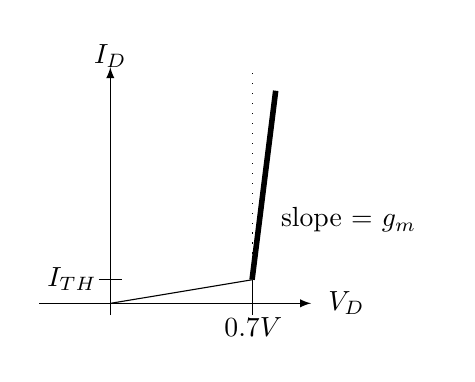
\begin{tikzpicture}[scale=0.6]
			\draw[line width=2pt] (5, 1.5) -- (5.5, 5.5);
			\draw[-latex] (1.5, 1) |- (6.25, 1);
			\draw[-latex] (2, 0.75) -| (2, 5.999);
			\draw (2, 0.999) -| (5, 1.498);
			\node[shape=rectangle, minimum width=1.09cm, minimum height=0.465cm] at (6.812, 1){} node[anchor=west, align=left, text width=0.702cm, inner sep=6pt] at (6.25, 1){$V_D$};
			\node[shape=rectangle, minimum width=1.09cm, minimum height=0.485cm] at (2, 6.239){} node[anchor=center, align=center, text width=0.702cm, inner sep=6pt] at (2, 6.239){$I_D$};
			\draw (5, 0.749) -- (5, 1.249);
			\node[shape=rectangle, minimum width=1.09cm, minimum height=0.485cm] at (5, 0.489){} node[anchor=center, align=center, text width=0.702cm, inner sep=6pt] at (5, 0.489){$0.7V$};
			\draw (1.75, 1.498) -- (2.25, 1.498);
			\node[shape=rectangle, minimum width=1.09cm, minimum height=0.485cm] at (1.187, 1.509){} node[anchor=center, align=center, text width=0.702cm, inner sep=6pt] at (1.187, 1.509){$I_{TH}$};
			\draw[dash pattern={on 0.4pt off 1.6pt}] (5, 1) -| (5, 1.498);
			\draw[dash pattern={on 0.4pt off 3.2pt}] (5, 1) -- (5, 6);
			\draw (2, 0.999) -- (5, 1.498);
			\draw (0.5, 1) -- (2, 1);
			\node[shape=rectangle, minimum width=2.277cm, minimum height=0.936cm] at (6.406, 2.765){} node[anchor=west, align=left, text width=1.889cm, inner sep=6pt] at (5.25, 2.765){slope = $g_m$};
		\end{tikzpicture}\\
		\hline
	\end{tabular}
\end{table}

In the most general case we don't know in what region the diode operates at, so $a$ and $b$ are unknown, but that is not an issue: the equation stays the same so we can carry on and solve for $V_D$ regardless:
$$
	V_D = V - RI_D = V - R \left( aV_D + b \right)
$$

%\fbox{$V_D = \dfrac{1}{1 + aR}V - \dfrac{bR}{1 + aR}$}

\centerline{\fbox{$V_D = \dfrac{1}{1 + aR}V - \dfrac{bR}{1 + aR}$}}

Now there are different interpretations depending on the bias point.  

\paragraph{Forward bias}\mbox{}\\

In particular, when $V \gg V_{TH}$, we can make the hypothesis that the diode is in Forward mode. We get:
$$
	V_D = \dfrac{1}{1 + g_mR}V + \dfrac{g_mR}{1 + g_mR}V_{TH} - \dfrac{RI_{TH}}{1 + g_mR}
$$

The specific feature of the Forward operating mode is that the transconductance $g_m$ is particularly high, which makes several terms negligible. So finally:

\centerline{\fbox{$V_D \simeq V_{TH}$}}

We've found a very common result: the diode voltage does not depend on the polarisation voltage $V$ anymore.

The analysis is not complete though, and only one direction of the implication was done:
$$
	 \text{initial conditions } (V, R) \Rightarrow D \text{ is in Forward mode}
$$

Strictly speaking, we would have to check that $D$ being in forward mode is compatible with these conditions.


\paragraph{"Weak Forward" bias}\mbox{}\\

The previous linearised equations allows us to study what happens in a less common case: the diode is below its conduction threshold.

From
$$
	V_D = \dfrac{1}{1 + aR}V - \dfrac{bR}{1 + aR}
$$

and since $b = 0$, we now get:
$$
	V_D \simeq V
$$

But that would be equivalent to say that the diode doesn't conduct at all.

Using the fact that $a \ll 1$, a less \textit{crude} approximation would give:
$$
	V_D = (1 - aR)V
$$



\section*{Example 2: Diode and Resistor II}
This is a slight variation of the previous diode circuit.\\

We now have a varying voltage source as input of the system, the diode voltage is the output. We want to see how the output varies with the input (assuming no current is drawn from the output).

\begin{circuitikz}
	\node[eground2] at (2, 1){};
	\draw (2, 2.5) to[empty diode, l={$D$}] (2, 1);
	\draw (2, 4.5) to[american resistor, /tikz/circuitikz/bipoles/length=1.05cm, l={$R$}] (2, 2.5);
	\draw (2, 4.5) |- (1, 5);
	\node[ocirc](N1) at (1, 5){} node[anchor=east] at (N1.west){$V_{IN}$};
	\draw[line width=1.6pt, -latex] (2, 4.5) -- (2, 4.25);
	\node[shape=rectangle, minimum width=0.715cm, minimum height=1.215cm] at (2.5, 4.375){} node[anchor=center, align=center, text width=0.327cm, inner sep=6pt] at (2.5, 4.375){$I_D$};
	\draw (2, 2.5) -- (3, 2.5);
	\node[circ] at (2, 2.5){};
	\node[ocirc](N2) at (3, 2.5){} node[anchor=west] at (N2.east){$V_{OUT}$};
\end{circuitikz}

In Forward mode, recall that:
$$
	V_D = \dfrac{1}{1 + g_mR}V_{IN} + \dfrac{g_mR}{1 + g_mR}V_{TH} - \dfrac{RI_{TH}}{1 + g_mR}
$$

If $V_{IN}$ is a constant value on top of which we apply some small deviation $\Delta V$ then  $V_{IN} = V_0 + \Delta V$ and:
$$
	\Delta V_D = \dfrac{1}{1 + g_mR}\Delta V
$$ 

It makes sense: for an increasing $V_{IN}$, the diode voltage cannot follow the input and rise as much: the exponential law would kick in and cause a massive increase in current, thereby reducing the diode voltage (through the resistor), opposing the initial voltage increase. 

In a way, the diode voltage \textbf{does not} want to change. It is the basis principle of Zener diode voltage regulators (although it makes the diode work in a different region —reverse breakdown— but the consequences are exactly the same).

Can we be more precise in the way the output gets regulated? Like before, if we just assume $V_D = 0.7V$, there's not much to say.
This is where the Piecewise Linear model can become handy. 

*** SECTION IS TODO *** .



\section*{Example 3: diode and resistor III}
Another variation on a theme of a Diode and Resistor circuit. This time, we swap the roles for the diode and resistor, and the output current is not neglected anymore.

\begin{circuitikz}
	\node[eground2] at (7, 6.75){};
	\draw (9, 11.25) to[american resistor, l={$R_1$}] (9, 9);
	\draw (9, 8.5) to[empty diode, l={$D$}] (9, 7);
	\node[ocirc](N1) at (7, 11.5){} node[anchor=east] at ([xshift=-0.08cm]N1.text){$V_{IN}$};
	\draw (7, 11.5) -- (9, 11.5) -- (9, 11.25);
	\node[ocirc](N2) at (11, 9){} node[anchor=west] at ([xshift=0.08cm]N2.text){$V_{OUT}$};
	\draw (11, 9) -- (9, 9);
	\node[circ] at (9, 9){};
	\draw (7, 9) to[american resistor, l={$R_2$}] (7, 6.75);
	\node[eground2] at (9, 6.75){};
	\draw (9, 6.75) -| (9, 7);
	\draw (9, 8.5) -| (9, 9);
	\draw (7, 9) -- (9, 9);
\end{circuitikz}



\section*{Example 4: the Common Collector (or \textit{Emitter Follower})}

Now moving onto applications of Bipolar Junction Transistors (BJT), let's study one of the most basic linear application of it.

\begin{circuitikz}
	\node[npn, tr circle](N1) at (12, 10.001){} node[anchor=west] at (N1.text){$Q_1$};
	\draw (12, 9.25) to[american resistor, /tikz/circuitikz/bipoles/length=0.700cm, l={$R_E$}] (12, 6.96);
	\node[eground2] at (12, 6.96){};
	\draw (13.5, 9) -- (12, 9);
	\draw (11.16, 10.001) |- (10, 10);
	\draw (12, 10.75) -- (12, 11.5);
	\node[vcc] at (12, 11.5){};
	\node[ocirc](N2) at (10, 10){} node[anchor=east] at (N2.text){$V_{IN}$};
	\node[ocirc](N3) at (13.5, 9){} node[anchor=west] at (N3.text){$V_{OUT}$};
	\node[circ] at (12, 9){};
\end{circuitikz}


The Common Collector Circuit helps isolating the input voltage from its output.


\subsubsection*{Transfert function}
For the BJT, we use the following model:

\begin{circuitikz}
	\draw[dash pattern={on 0.4pt off 3.2pt}] (2, -0.75) -| (2, 8);
	\draw[-latex] (1, 0.999) -- (7, 0.999);
	\draw[-latex] (2, -0.001) -- (2, 5.999);
	\draw[line width=1.9pt] (2, 0.999) -- (0.25, 0.999);
	\draw[line width=2pt] (2, 0.999) -- (5, 1.499);
	\draw[line width=2pt] (5, 1.499) -- (6, 5.499);
	\node[shape=rectangle, minimum width=1.09cm, minimum height=0.985cm] at (7.563, 1.009){} node[anchor=west, align=left, text width=0.702cm, inner sep=6pt] at (7, 1.009){$V_{BE}$};
	\node[shape=rectangle, minimum width=1.09cm, minimum height=0.485cm] at (2, 6.239){} node[anchor=center, align=center, text width=0.702cm, inner sep=6pt] at (2, 6.239){$I_C$};
	\draw (5, 0.749) -- (5, 1.249);
	\node[shape=rectangle, minimum width=1.09cm, minimum height=0.485cm] at (5, 0.489){} node[anchor=center, align=center, text width=0.702cm, inner sep=6pt] at (5, 0.489){$0.7V$};
	\draw (1.75, 1.499) -- (2.25, 1.499);
	\node[shape=rectangle, minimum width=1.09cm, minimum height=0.485cm] at (1.187, 1.509){} node[anchor=center, align=center, text width=0.702cm, inner sep=6pt] at (1.187, 1.509){$I_{TH}$};
	\draw (5.25, 2.499) -- (5.75, 2.499) -- (5.75, 4.499);
	\node[shape=rectangle, minimum width=0.652cm, minimum height=1.965cm] at (6.156, 3.499){} node[anchor=center, align=center, text width=0.264cm, inner sep=6pt] at (6.156, 3.499){$g_{m}$};
	\node[shape=rectangle, minimum width=0.84cm, minimum height=0.485cm] at (5.562, 2.239){} node[anchor=center, align=center, text width=0.452cm, inner sep=6pt] at (5.562, 2.239){$1$};
	\draw[dash pattern={on 0.4pt off 1.6pt}] (2, 1.5) -| (5, 1.499);
	\draw[dash pattern={on 0.4pt off 1.6pt}] (5, 1) -| (5, 1.499);
	\node[shape=rectangle, minimum width=1.715cm, minimum height=0.465cm] at (1.125, 7.25){} node[anchor=center, align=center, text width=1.327cm, inner sep=6pt] at (1.125, 7.25){Reverse};
	\node[shape=rectangle, minimum width=2.965cm, minimum height=0.465cm] at (3.5, 7.25){} node[anchor=center, align=center, text width=2.577cm, inner sep=6pt] at (3.5, 7.25){Cutoff};
	\node[shape=rectangle, minimum width=1.965cm, minimum height=0.965cm] at (6, 7.25){} node[anchor=center, align=center, text width=1.577cm, inner sep=6pt] at (6, 7.25){Forward Active};
	\draw[dash pattern={on 0.4pt off 3.2pt}] (5, -0.75) -| (5, 8);
	\draw[dash pattern={on 0.4pt off 3.2pt}] (7, -0.75) -| (7, 8);
\end{circuitikz}

As we will see, for the common collector, the actual values for $g_m$ and $I_{TH}$ do not matter that much. However, this is not true in the general case. We will illustrate that in later examples.\\


So just like we did with the diode previously: we assume a linear model $I_C = f(V_{BE}) = a V_{BE} + b$ with $a$ and $b$ depending on the operating point (Reverse, Cutoff, Forward Active).

$$
	V_{OUT} = R_E f(V_{IN} - V_{OUT}) = a R_E \left(V_{IN} - V_{OUT} \right) + b
$$

Rearranging for $V_{OUT}$:

\fbox{$V_{OUT} = \dfrac{a R_E}{1 + a R_E} V_{IN} + \dfrac{b}{1 + a R_E}$}



\subsubsection*{A BJT is an op amp in disguise.}
We've just seen that a BJT in the common emitter arrangement is basically always 'on'. It's the very high transconductance past the $V_{BE} = 0.7V$ that makes all the system work.\\
Applying a very high gain to a voltage difference reminds us of op amps. Under the hood, an op amp is voltage difference amplifier with a massive gain ($>10^6$)\\
The high gain is rarely used as such because it is not very predictable, controlled and uniform in frequency. 
We much prefer to use this 'unreliable' gain in a feedback loop. It reduces the amplification, but it is more robust to part to part fluctuation

\subsubsection*{Input Impedance}
*** SECTION IS TODO *** .



\section*{Example 5: the Rubber Diode}

\subsubsection*{Description}
In a Class AB Amplifier, we need to 'pre-heat' the NPN and PNP transistors of the final stage.
This allows a quiescent current to flow at rest and maintain both transistor in active region. 
It is mandatory to get rid of the \textit{crossover distortion}.\\

The polarisation is done usually with 2 diodes in series. 
But for more flexibility, one can also use the \textit{Rubber Diode} below.\\

It is quite common to have a potentiometer for the resistors $R_1$ and $R_2$ to fine-tune the voltage $V$.\\

\begin{circuitikz}
	\draw (2.25, 4.5) -- (2.25, 3.75);
	\node[npn, tr circle] at (3, 2){};
	\draw[-latex] (4.5, -0.5) -- (4.5, 4.5);
	\node[shape=rectangle, minimum width=0.715cm, minimum height=4.965cm] at (4.875, 2){} node[anchor=center, align=center, text width=0.327cm, inner sep=6pt] at (4.875, 2){$V$};
	\draw[line width=2pt, -latex] (2.25, 4.25) -- (2.25, 4);
	\node[shape=rectangle, minimum width=0.965cm, minimum height=0.715cm] at (2.75, 4.125){} node[anchor=north west, align=left, text width=0.577cm, inner sep=6pt] at (2.25, 4.5){$I$};
	\draw (1.5, 3.5) to[american resistor, /tikz/circuitikz/bipoles/length=0.700cm, l={$R_1$}] (1.5, 2.25);
	\draw (1.5, 1.75) to[american resistor, /tikz/circuitikz/bipoles/length=0.700cm, l={$R_2$}] (1.5, 0.5);
	\draw (1.5, 0.5) |- (3, 0.25) -| (3, 1.23);
	\draw (1.5, 3.5) -| (1.5, 3.75) -- (3, 3.75) -| (3, 2.75);
	\draw (1.5, 2.25) -| (1.5, 1.75);
	\draw (2.16, 2) -- (1.5, 2);
	\node[circ] at (1.5, 2){};
	\draw (2.25, 0.25) -- (2.25, -0.5);
	\node[circ] at (2.25, 3.75){};
	\node[circ] at (2.25, 0.25){};
	\node[ocirc] at (2.25, 4.5){};
	\node[ocirc] at (2.25, -0.5){};
	\draw[line width=2pt, -latex] (1.5, 3.5) -- (1.5, 3.25);
	\draw[line width=2pt, -latex] (3, 3.5) -- (3, 3.25);
	\node[shape=rectangle, minimum width=0.715cm, minimum height=0.715cm] at (1, 3.375){} node[anchor=north, align=center, text width=0.327cm, inner sep=6pt] at (1, 3.75){$I_R$};
	\draw[dash pattern={on 0.4pt off 1.6pt}] (2.5, 4.5) -- (5, 4.5);
	\draw[dash pattern={on 0.4pt off 1.6pt}] (2.5, -0.5) -- (5, -0.5);
	\node[shape=rectangle, minimum width=0.715cm, minimum height=0.715cm] at (3.5, 3.375){} node[anchor=north, align=center, text width=0.327cm, inner sep=6pt] at (3.5, 3.75){$I_C$};
\end{circuitikz}

\subsubsection*{Derivation}
Just like with the examples before, we can ignore the base current as a first approximation. Then:
\begin{equation}
\begin{split}
I & = I_R + I_C \\
 	& = \dfrac{V}{R_1 + R_2} + f \left( \dfrac{R_2}{R_1 + R_2} V \right)\\
	& = \dfrac{V}{R_1 + R_2} + a \dfrac{R_2}{R_1 + R_2} V + b\\
	& = \dfrac{1 + a R_2}{R_1 + R_2} V + b
\end{split}
\end{equation}

Therefore:

\centerline{\fbox{$V = \dfrac{R_1+R_2}{1+aR_2}\left(I-b\right)$}}

Iterating over the different possible modes, we get:

\begin{table}[h]
	\centering
	\begin{tabular}{|c||c|c|c|}
		\hline
		\textbf{BJT mode} & \textbf{Gain/Offset} & $V = f(I)$ \\ \hline

		Reverse 
		& 
		$\left\{
		\begin{array}{ll}
			a = 0 \\
			b = 0
		\end{array}
		\right.$
		& 
		$V = (R_1 + R_2)I$	\\ \hline

		Weak Forward
		& 
		$\left\{
		\begin{array}{ll}
			a = \frac{I_{TH}}{V_{TH}} \\
			b = 0
		\end{array}
		\right.$
		& 
		TODO 	\\ \hline

		Forward
		& 
		$\left\{
		\begin{array}{ll}
			a = g_m \\
			b = I_{TH}-g_m V_{TH}
		\end{array}
		\right.$ 
		&
		TODO 	\\ \hline
	\end{tabular}
\end{table}


We can now have a closer look at the behaviour for the different operating regions of the transistor:

\begin{table}[H]
	\centering
	\begin{tabular}{|m{1.5cm}||m{5cm}|m{6cm}|}
		\hline
		\textbf{BJT Mode} & \textbf{BJT Operating point} & \textbf{Rubber Diode} $V = f(I)$\\ \hline

		Reverse & 
		\begin{tikzpicture}
			\draw[-latex] (1, 1) -- (5, 1);
			\draw[-latex] (3, 0.75) -- (3, 3);
			\node[shape=rectangle, minimum width=0.965cm, minimum height=0.715cm](N1) at (5.5, 1){} node[anchor=center] at (N1.text){$V_{BE}$};
			\node[shape=rectangle, minimum width=0.965cm, minimum height=0.715cm](N2) at (3, 3.375){} node[anchor=center] at (N2.text){$I_C$};
			\draw[line width=2pt] (1, 1) -- (3, 1);
			\draw[dash pattern={on 0.4pt off 0.8pt}] (3, 1) -- (4.25, 1.25);
			\draw[dash pattern={on 0.4pt off 1.6pt}] (4.25, 1.25) -- (4.75, 3);
			\node[circ, xscale=1.2, yscale=1.2] at (3, 1){};
		\end{tikzpicture}
		& 
		\begin{tikzpicture}
			\draw[-latex] (8, 1) -- (13, 1);
			\draw[-latex] (9, 0.75) -- (9, 3);
			\node[shape=rectangle, minimum width=0.965cm, minimum height=0.715cm](N1) at (13.5, 1){} node[anchor=center] at (N1.text){$\Delta V$};
			\node[shape=rectangle, minimum width=0.965cm, minimum height=0.715cm](N2) at (9, 3.375){} node[anchor=center] at (N2.text){$I_S$};
			\draw[line width=2pt] (11, 1) -- (12.75, 1);
			\node[circ, xscale=1.2, yscale=1.2] at (11, 1){};
			\draw (11, 0.75) -- (11, 1.25);
			\draw (9.25, 0.75) -- (9.25, 1.25);
			\node[shape=rectangle, minimum width=0.465cm, minimum height=0.84cm](N3) at (11, 0.187){} node[anchor=center] at (N3.text){$\dfrac{V_B}{2}$};
			\node[shape=rectangle, minimum width=2.465cm, minimum height=0.965cm](N4) at (9.25, -0.5){} node[anchor=center] at (N4.text){$\dfrac{V_B}{2}-V_{TH}$};
			\draw (8.75, 0.157) -- (9.25, 0.657);
			\draw[dash pattern={on 0.4pt off 1.6pt}] (11, 1) -- (9.25, 1.5);
			\draw[dash pattern={on 0.4pt off 1.6pt}] (9.25, 1.5) -- (8.25, 3.5);
		\end{tikzpicture} \\ \hline

		Weak Forward &
		\begin{tikzpicture}
			\draw[-latex] (1, 1) -- (5, 1);
			\draw[-latex] (3, 0.75) -- (3, 3);
			\node[shape=rectangle, minimum width=0.965cm, minimum height=0.715cm](N1) at (5.5, 1){} node[anchor=center] at (N1.text){$V_{BE}$};
			\node[shape=rectangle, minimum width=0.965cm, minimum height=0.715cm](N2) at (3, 3.375){} node[anchor=center] at (N2.text){$I_C$};
			\draw[line width=2pt] (3, 1) -- (4.25, 1.25);
			\draw[dash pattern={on 0.4pt off 1.6pt}] (4.25, 1.25) -- (4.75, 3);
			\node[circ, xscale=1.2, yscale=1.2] at (3, 1){};
			\draw[dash pattern={on 0.4pt off 1.6pt}] (1, 1.006) -- (3, 1.006);
			\node[circ, xscale=1.2, yscale=1.2] at (4.25, 1.25){};
		\end{tikzpicture}
		& 
		\begin{tikzpicture}
			\draw (11, 0.75) -- (11, 1.25);
			\draw[-latex] (8, 1) -- (13, 1);
			\draw[-latex] (9, 0.75) -- (9, 3);
			\node[shape=rectangle, minimum width=0.965cm, minimum height=0.715cm](N1) at (13.5, 1){} node[anchor=center] at (N1.text){$\Delta V$};
			\node[shape=rectangle, minimum width=0.965cm, minimum height=0.715cm](N2) at (9, 3.375){} node[anchor=center] at (N2.text){$I_S$};
			\draw[dash pattern={on 0.4pt off 1.6pt}] (11, 1) -- (12.75, 1);
			\node[circ, xscale=1.2, yscale=1.2] at (11, 1){};
			\draw (9.25, 0.75) -- (9.25, 1.25);
			\node[shape=rectangle, minimum width=0.465cm, minimum height=0.84cm](N3) at (11, 0.187){} node[anchor=center] at (N3.text){$\dfrac{V_B}{2}$};
			\node[shape=rectangle, minimum width=2.465cm, minimum height=0.965cm](N4) at (9.25, -0.5){} node[anchor=center] at (N4.text){$\dfrac{V_B}{2}-V_{TH}$};
			\draw (8.75, 0.157) -- (9.25, 0.657);
			\draw[line width=2pt] (11, 1) -- (9.25, 1.5);
			\draw[dash pattern={on 0.4pt off 1.6pt}] (9.25, 1.5) -- (8.25, 3.5);
			\node[circ, xscale=1.2, yscale=1.2] at (9.25, 1.5){};
		\end{tikzpicture} \\ \hline

		Forward & 
		\begin{tikzpicture}
			\draw[-latex] (1, 1) -- (5, 1);
			\draw[-latex] (3, 0.75) -- (3, 3);
			\node[shape=rectangle, minimum width=0.965cm, minimum height=0.715cm](N1) at (5.5, 1){} node[anchor=center] at (N1.text){$V_{BE}$};
			\node[shape=rectangle, minimum width=0.965cm, minimum height=0.715cm](N2) at (3, 3.375){} node[anchor=center] at (N2.text){$I_C$};
			\draw[dash pattern={on 0.4pt off 1.6pt}] (3, 1) -- (4.25, 1.25);
			\draw[line width=2pt] (4.25, 1.25) -- (4.75, 3);
			\node[circ, xscale=1.2, yscale=1.2] at (4.75, 3){};
			\draw[dash pattern={on 0.4pt off 1.6pt}] (1, 1) -- (3, 1);
			\node[circ, xscale=1.2, yscale=1.2] at (4.25, 1.25){};
		\end{tikzpicture}
		& 
		\begin{tikzpicture}
			\draw (11, 0.75) -- (11, 1.25);
			\draw[-latex] (8, 1) -- (13, 1);
			\draw[-latex] (9, 0.75) -- (9, 3);
			\node[shape=rectangle, minimum width=0.965cm, minimum height=0.715cm](N1) at (13.5, 1){} node[anchor=center] at (N1.text){$\Delta V$};
			\node[shape=rectangle, minimum width=0.965cm, minimum height=0.715cm](N2) at (9, 3.375){} node[anchor=center] at (N2.text){$I_S$};
			\draw[dash pattern={on 0.4pt off 1.6pt}] (11, 1) -- (12.75, 1);
			\draw (9.25, 0.75) -- (9.25, 1.25);
			\node[shape=rectangle, minimum width=0.465cm, minimum height=0.84cm](N3) at (11, 0.187){} node[anchor=center] at (N3.text){$\dfrac{V_B}{2}$};
			\node[shape=rectangle, minimum width=2.465cm, minimum height=0.965cm](N4) at (9.25, -0.5){} node[anchor=center] at (N4.text){$\dfrac{V_B}{2}-V_{TH}$};
			\draw (8.75, 0.157) -- (9.25, 0.657);
			\draw[dash pattern={on 0.4pt off 1.6pt}] (11, 1) -- (9.25, 1.5);
			\draw[line width=2pt] (9.25, 1.5) -- (8.25, 3.5);
			\node[circ, xscale=1.2, yscale=1.2] at (9.25, 1.5){};
			\node[circ, xscale=1.2, yscale=1.2] at (8.25, 3.5){};
		\end{tikzpicture} \\ \hline
	\end{tabular}
\end{table}




A few observations:
\begin{itemize}
	\item starts to act as a diode when $\frac{R_2}{R_1+R_2} \simeq 0.7V$
	\item when active, the new transconductance becomes $\hat{g}_m=\frac{1 + g_m R_2}{R_1+R_2}$
\end{itemize}


\section*{Example 6: the Class AB Amplifier}

The Class AB Amplifier (or \textit{Push-Pull}) is the typical output stage for many IC devices (op amps, audio amplifiers, etc.) It shows up anytime there is a need to drive a load with some power.

We present here below a simplified view of the circuit in its most general case (with emitter resistors). The polarisation stages are abstracted as simple voltage sources (it doesn't matter much for now).

\begin{circuitikz}
	\draw (4, 8.02) -| (4, 9);
	\draw (0.25, 5) -- (2, 5);
	\draw (4, 6.5) to[american resistor, /tikz/circuitikz/bipoles/length=0.700cm, l={$R_E$}] (4, 5.25);
	\node[npn, tr circle](N1) at (4, 7.25){} node[anchor=west] at (N1.text){$Q_1$};
	\node[pnp, tr circle](N2) at (4, 2.75){} node[anchor=west] at (N2.text){$Q_2$};
	\draw (4, 4.77) to[american resistor, /tikz/circuitikz/bipoles/length=0.700cm, l={$R_E$}] (4, 3.52);
	\draw (4, 4.77) -- (4, 5.25);
	\draw (2, 7) to[american voltage source, l={$V_B/2$}] (2, 5.5);
	\draw (2, 4.5) to[american voltage source, l={$V_B/2$}] (2, 3);
	\draw (3.16, 2.75) -| (2, 3);
	\draw (3.16, 7.25) -| (2, 7);
	\draw (2, 5.5) -| (2, 4.5);
	\node[ocirc](N3) at (4, 9){} node[anchor=south] at (N3.text){$+V_{CC}$};
	\draw (4, 1.98) -- (4, 1);
	\draw (4, 5) -| (5.75, 4.75);
	\draw (5.75, 4.75) to[american resistor, /tikz/circuitikz/bipoles/length=0.700cm, l={$R_L$}] (5.75, 3.5);
	\node[circ] at (4, 5){};
	\node[eground2] at (5.75, 3.5){};
	\node[circ] at (2, 5){};
	\node[ocirc](N4) at (0.25, 5){} node[anchor=east] at (N4.text){$V_{IN}$};
	\draw[line width=2pt, -latex] (4, 8.5) -- (4, 8.25);
	\node[shape=rectangle, minimum width=0.965cm, minimum height=0.715cm] at (4.5, 8.375){} node[anchor=north west, align=left, text width=0.577cm, inner sep=6pt] at (4, 8.75){$I_S$};
	\draw[line width=2pt, -latex] (4, 1.75) -- (4, 1.5);
	\node[shape=rectangle, minimum width=0.965cm, minimum height=0.715cm] at (4.5, 1.605){} node[anchor=north west, align=left, text width=0.577cm, inner sep=6pt] at (4, 1.98){$I_D$};
	\draw[-latex] (6.75, 3.5) -- (6.75, 4.75);
	\node[shape=rectangle, minimum width=0.965cm, minimum height=0.715cm] at (7.25, 4.125){} node[anchor=north west, align=left, text width=0.577cm, inner sep=6pt] at (6.75, 4.5){$V_{OUT}$};
	\node[ocirc](N5) at (4, 1){} node[anchor=north] at (N5.text){$-V_{CC}$};
	\draw[dash pattern={on 0.4pt off 1.6pt}] (5.75, 5) -- (7, 5);
\end{circuitikz}

\paragraph{Derivation}\mbox{}\\
We assume that the base current are negligible. 

We denote the collector currents as $I_C = f_S(V_{BE})$ for the NPN and $I_C = f_D(V_{EB})$ for the PNP. 

$V_B$ (the bias voltage) is usually around $2V_{BE} \simeq 1.4V$ or above. 

$V_{IN}$ is the amplifier's input voltage, we treat it as a static voltage source and we will try to derive the output voltage from it. 

We focus on audio applications, so as  first approximation the load $R_L$ is essentially ohmic, and usually low impedance (8 to 32 $\Omega$ range).

Then, applying the usual KVL and KCL:
$$
\left\{
	\begin{array}{ll}
		I_S = f_S \left(V_{IN} - V_{OUT} + \dfrac{V_B}{2} - R_E I_S \right) \\
		I_D = f_D \left(-(V_{OUT} - V_{IN}) + \dfrac{V_B}{2} - R_E I_D \right) \\
		V_{OUT} = R_L(I_S-I_D)
	\end{array}
\right.
$$\\

This time, the equations are trickier: the unknowns $I_S$, $I_D$ and $V_{OUT}$ are all intertwined.
$I_S$ depends on $I_S$ (feedback) and $V_{OUT}$, but $V_{OUT}$ itself depends on $I_S$...\\

To solve it, we can first try to simplify the whole schematic and see it as being made out of 2 independant subsystems:

\begin{circuitikz}
	\draw (1, 5) -| (2, 5);
	\draw (4, 4.25) -- (4, 5.75);
	\draw (2, 5.75) -| (2, 4.25);
	\draw (4, 5) -| (5.75, 4.75);
	\draw (5.75, 4.75) to[american resistor, /tikz/circuitikz/bipoles/length=0.700cm, l={$R_L$}] (5.75, 3.5);
	\node[circ] at (4, 5){};
	\node[eground2] at (5.75, 3.5){};
	\node[circ] at (2, 5){};
	\node[ocirc](N1) at (1, 5){} node[anchor=east] at (N1.text){$V_{IN}$};
	\draw[-latex] (6.75, 3.5) -- (6.75, 4.75);
	\node[shape=rectangle, minimum width=0.965cm, minimum height=0.715cm] at (7.25, 4.125){} node[anchor=north west, align=left, text width=0.577cm, inner sep=6pt] at (6.75, 4.5){$V_{OUT}$};
	\draw[dash pattern={on 0.4pt off 1.6pt}] (5.75, 5) -- (7, 5);
	\node[shape=rectangle, draw, line width=1pt, minimum width=2.965cm, minimum height=1.465cm] at (3, 6.5){} node[anchor=center, align=center, text width=2.577cm, inner sep=6pt] at (3, 6.5){Source subsystem};
	\node[shape=rectangle, draw, line width=1pt, minimum width=2.965cm, minimum height=1.465cm] at (3, 3.5){} node[anchor=center, align=center, text width=2.577cm, inner sep=6pt] at (3, 3.5){Drain subsystem};
	\draw[line width=1pt, -latex] (2.25, 5) -- (3.75, 5);
	\node[shape=rectangle, minimum width=0.965cm, minimum height=0.715cm] at (3, 4.625){} node[anchor=north west, align=left, text width=0.577cm, inner sep=6pt] at (2.5, 5){$\Delta V$};
	\draw[line width=1.5pt, -latex] (4, 5.5) -| (4, 5.25);
	\draw[line width=1.5pt, -latex] (4, 4.75) -| (4, 4.5);
	\node[shape=rectangle, minimum width=0.965cm, minimum height=0.715cm] at (4.5, 5.375){} node[anchor=north west, align=left, text width=0.577cm, inner sep=6pt] at (4, 5.75){$I_S$};
	\node[shape=rectangle, minimum width=0.965cm, minimum height=0.715cm] at (4.5, 4.625){} node[anchor=north west, align=left, text width=0.577cm, inner sep=6pt] at (4, 5){$I_D$};
	\draw[line width=1.5pt, -latex] (5.25, 5) -- (5.5, 5);
	\node[shape=rectangle, minimum width=0.965cm, minimum height=0.715cm] at (5.5, 5.375){} node[anchor=north west, align=left, text width=0.577cm, inner sep=6pt] at (5, 5.75){$I_L$};
\end{circuitikz}

Now we can focus on each system and solve them individually.

%Therefore, the overall behaviour can be derived from the behaviour of these two subsystems that only depend on an input voltage $\Delta V = %V_{OUT} - V_{IN}$

\subsection*{Class AB subsystem: the current source}
Following the way we split the schematic, the Source Subsystem would look like this:\\

\begin{circuitikz}
	\draw[dash pattern={on 0.4pt off 1.6pt}] (5, -0.75) |- (4, -0.75);
	\draw[dash pattern={on 0.4pt off 1.6pt}] (5, 0.5) |- (4, 0.5);
	\draw (4, 2.48) -- (4, 0.5);
	\node[shape=rectangle, draw, line width=1pt, dash pattern={on 1pt off 4pt}, minimum width=4.215cm, minimum height=4.715cm] at (3.375, 4.125){};
	\draw (4, 3.73) to[american resistor, /tikz/circuitikz/bipoles/length=0.700cm, l={$R_E$}] (4, 2.48);
	\node[npn, tr circle](N1) at (4, 4.48){} node[anchor=west] at ([xshift=0.13cm]N1.text){$Q_1$};
	\draw (2, 4.23) to[american voltage source, l={$V_B/2$}] (2, 2.73);
	\draw (3.16, 4.48) -| (2, 4.23);
	\draw (4, 5.27) -- (4, 5.75);
	\node[eground2] at (4, -0.75){};
	\node[ocirc] at (4, -0.75){};
	\draw[line width=2pt, -latex] (4, 1.25) -- (4, 1);
	\draw[line width=1pt, -latex] (4.5, -0.75) -- (4.5, 0.5);
	\node[shape=rectangle, minimum width=0.84cm, minimum height=0.715cm] at (4.937, -0.125){} node[anchor=north, align=center, text width=0.452cm, inner sep=6pt] at (4.937, 0.25){$\Delta V$};
	\node[ocirc] at (4, 0.5){};
	\node[shape=rectangle, minimum width=0.965cm, minimum height=0.715cm] at (4.5, 1.125){} node[anchor=north west, align=left, text width=0.577cm, inner sep=6pt] at (4, 1.5){$I_S$};
	\node[eground2] at (2, 2.73){};
	\node[ocirc](N2) at (4, 5.75){} node[anchor=south] at (N2.text){$+V_{CC}$};
\end{circuitikz}

The source current $I_S$ is then expressed as:
$$
I_S = f_S \left(-\Delta V + \dfrac{V_B}{2} - R_E I_S \right) \\
$$

Under a linear model assumption $f_S(V) = aV+b$, we can write that:
$$
	I_S = a \left(-\Delta V + \dfrac{V_B}{2} - R_E I_S \right) + b
$$

Finally, after a bit of algebra:

\fbox{$I_S = -\dfrac{1}{R_E}\dfrac{a R_E}{1+a R_E}\Delta V + \dfrac{a \frac{V_B}{2} + b}{1 + a R_E} \triangleq \hat{f}_S (\Delta V)$}

We can treat the Source Subsystem as a \textit{virtual} device with its own $I_S = \hat{f}_S (\Delta V)$ transfer curve. And since we assumed a piecewise linear model for the BJT, this device exhibits a piecewise linear characteristic curve too.

To explicit it, let's apply a voltage $\Delta V$ in the range $-2.0V ... 2.0V$, evaluate $I_S$ using the equation above and pick the gain/offset pair $(a(\Delta V), b(\Delta V))$ that works.

\begin{table}[h]
	\centering
	\begin{tabular}{|c||c|c|c|}
		\hline
		\textbf{BJT mode} & \textbf{Gain/Offset} & $I_S = \hat{f}_S (\Delta V)$ \\ \hline

		Reverse 
		& 
		$\left\{
		\begin{array}{ll}
			a = 0 \\
			b = 0
		\end{array}
		\right.$
		& 
		$I_S(\Delta V) = 0$	\\ \hline

		Weak Forward
		& 
		$\left\{
		\begin{array}{ll}
			a = \frac{I_{TH}}{V_{TH}} \\
			b = 0
		\end{array}
		\right.$
		& 
		$I_S(\Delta V) = \dfrac{-a}{1+aR_E} \left( \Delta V-\dfrac{V_B}{2} \right)$	\\ \hline

		Forward
		& 
		$\left\{
		\begin{array}{ll}
			a = g_m \\
			b = I_{TH}-g_m V_{TH}
		\end{array}
		\right.$ 
		&
		$I_S(\Delta V) = \dfrac{-g_m}{1+g_mR_E} \left(\dfrac{V_B}{2} - \Delta V + I_{TH} - gmV_{TH} \right) $\\ \hline
	\end{tabular}
\end{table}

Using continuity at $V_{BE} = V_{TH}$, we can determine the voltage $\Delta V^F$ where the source subsystem makes $Q_1$ to go from Weak Forward to Forward mode:
$$
	\Delta V^F = \dfrac{V_B}{2} - \dfrac{1}{1-\dfrac{aR_E}{1+aR_E}} V_{TH} \simeq \dfrac{V_B}{2} - V_{TH}
$$

In practical applications, $V_B \simeq 2 V_{TH}$, therefore $\Delta V^F \simeq 0$.

\begin{table}[H]
	\centering
	\begin{tabular}{|m{1.5cm}||m{5cm}|m{6cm}|}
		\hline
		BJT Mode & BJT Operating point & Source Subsystem \\ \hline

		Reverse & 
		\begin{tikzpicture}
			\draw[-latex] (1, 1) -- (5, 1);
			\draw[-latex] (3, 0.75) -- (3, 3);
			\node[shape=rectangle, minimum width=0.965cm, minimum height=0.715cm](N1) at (5.5, 1){} node[anchor=center] at (N1.text){$V_{BE}$};
			\node[shape=rectangle, minimum width=0.965cm, minimum height=0.715cm](N2) at (3, 3.375){} node[anchor=center] at (N2.text){$I_C$};
			\draw[line width=2pt] (1, 1) -- (3, 1);
			\draw[dash pattern={on 0.4pt off 0.8pt}] (3, 1) -- (4.25, 1.25);
			\draw[dash pattern={on 0.4pt off 1.6pt}] (4.25, 1.25) -- (4.75, 3);
			\node[circ, xscale=1.2, yscale=1.2] at (3, 1){};
		\end{tikzpicture}
		& 
		\begin{tikzpicture}
			\draw[-latex] (8, 1) -- (13, 1);
			\draw[-latex] (9, 0.75) -- (9, 3);
			\node[shape=rectangle, minimum width=0.965cm, minimum height=0.715cm](N1) at (13.5, 1){} node[anchor=center] at (N1.text){$\Delta V$};
			\node[shape=rectangle, minimum width=0.965cm, minimum height=0.715cm](N2) at (9, 3.375){} node[anchor=center] at (N2.text){$I_S$};
			\draw[line width=2pt] (11, 1) -- (12.75, 1);
			\node[circ, xscale=1.2, yscale=1.2] at (11, 1){};
			\draw (11, 0.75) -- (11, 1.25);
			\draw (9.25, 0.75) -- (9.25, 1.25);
			\node[shape=rectangle, minimum width=0.465cm, minimum height=0.84cm](N3) at (11, 0.187){} node[anchor=center] at (N3.text){$\dfrac{V_B}{2}$};
			\node[shape=rectangle, minimum width=2.465cm, minimum height=0.965cm](N4) at (9.25, -0.5){} node[anchor=center] at (N4.text){$\dfrac{V_B}{2}-V_{TH}$};
			\draw (8.75, 0.157) -- (9.25, 0.657);
			\draw[dash pattern={on 0.4pt off 1.6pt}] (11, 1) -- (9.25, 1.5);
			\draw[dash pattern={on 0.4pt off 1.6pt}] (9.25, 1.5) -- (8.25, 3.5);
		\end{tikzpicture} \\ \hline

		Weak Forward &
		\begin{tikzpicture}
			\draw[-latex] (1, 1) -- (5, 1);
			\draw[-latex] (3, 0.75) -- (3, 3);
			\node[shape=rectangle, minimum width=0.965cm, minimum height=0.715cm](N1) at (5.5, 1){} node[anchor=center] at (N1.text){$V_{BE}$};
			\node[shape=rectangle, minimum width=0.965cm, minimum height=0.715cm](N2) at (3, 3.375){} node[anchor=center] at (N2.text){$I_C$};
			\draw[line width=2pt] (3, 1) -- (4.25, 1.25);
			\draw[dash pattern={on 0.4pt off 1.6pt}] (4.25, 1.25) -- (4.75, 3);
			\node[circ, xscale=1.2, yscale=1.2] at (3, 1){};
			\draw[dash pattern={on 0.4pt off 1.6pt}] (1, 1.006) -- (3, 1.006);
			\node[circ, xscale=1.2, yscale=1.2] at (4.25, 1.25){};
		\end{tikzpicture}
		& 
		\begin{tikzpicture}
			\draw (11, 0.75) -- (11, 1.25);
			\draw[-latex] (8, 1) -- (13, 1);
			\draw[-latex] (9, 0.75) -- (9, 3);
			\node[shape=rectangle, minimum width=0.965cm, minimum height=0.715cm](N1) at (13.5, 1){} node[anchor=center] at (N1.text){$\Delta V$};
			\node[shape=rectangle, minimum width=0.965cm, minimum height=0.715cm](N2) at (9, 3.375){} node[anchor=center] at (N2.text){$I_S$};
			\draw[dash pattern={on 0.4pt off 1.6pt}] (11, 1) -- (12.75, 1);
			\node[circ, xscale=1.2, yscale=1.2] at (11, 1){};
			\draw (9.25, 0.75) -- (9.25, 1.25);
			\node[shape=rectangle, minimum width=0.465cm, minimum height=0.84cm](N3) at (11, 0.187){} node[anchor=center] at (N3.text){$\dfrac{V_B}{2}$};
			\node[shape=rectangle, minimum width=2.465cm, minimum height=0.965cm](N4) at (9.25, -0.5){} node[anchor=center] at (N4.text){$\dfrac{V_B}{2}-V_{TH}$};
			\draw (8.75, 0.157) -- (9.25, 0.657);
			\draw[line width=2pt] (11, 1) -- (9.25, 1.5);
			\draw[dash pattern={on 0.4pt off 1.6pt}] (9.25, 1.5) -- (8.25, 3.5);
			\node[circ, xscale=1.2, yscale=1.2] at (9.25, 1.5){};
		\end{tikzpicture} \\ \hline

		Forward & 
		\begin{tikzpicture}
			\draw[-latex] (1, 1) -- (5, 1);
			\draw[-latex] (3, 0.75) -- (3, 3);
			\node[shape=rectangle, minimum width=0.965cm, minimum height=0.715cm](N1) at (5.5, 1){} node[anchor=center] at (N1.text){$V_{BE}$};
			\node[shape=rectangle, minimum width=0.965cm, minimum height=0.715cm](N2) at (3, 3.375){} node[anchor=center] at (N2.text){$I_C$};
			\draw[dash pattern={on 0.4pt off 1.6pt}] (3, 1) -- (4.25, 1.25);
			\draw[line width=2pt] (4.25, 1.25) -- (4.75, 3);
			\node[circ, xscale=1.2, yscale=1.2] at (4.75, 3){};
			\draw[dash pattern={on 0.4pt off 1.6pt}] (1, 1) -- (3, 1);
			\node[circ, xscale=1.2, yscale=1.2] at (4.25, 1.25){};
		\end{tikzpicture}
		& 
		\begin{tikzpicture}
			\draw (11, 0.75) -- (11, 1.25);
			\draw[-latex] (8, 1) -- (13, 1);
			\draw[-latex] (9, 0.75) -- (9, 3);
			\node[shape=rectangle, minimum width=0.965cm, minimum height=0.715cm](N1) at (13.5, 1){} node[anchor=center] at (N1.text){$\Delta V$};
			\node[shape=rectangle, minimum width=0.965cm, minimum height=0.715cm](N2) at (9, 3.375){} node[anchor=center] at (N2.text){$I_S$};
			\draw[dash pattern={on 0.4pt off 1.6pt}] (11, 1) -- (12.75, 1);
			\draw (9.25, 0.75) -- (9.25, 1.25);
			\node[shape=rectangle, minimum width=0.465cm, minimum height=0.84cm](N3) at (11, 0.187){} node[anchor=center] at (N3.text){$\dfrac{V_B}{2}$};
			\node[shape=rectangle, minimum width=2.465cm, minimum height=0.965cm](N4) at (9.25, -0.5){} node[anchor=center] at (N4.text){$\dfrac{V_B}{2}-V_{TH}$};
			\draw (8.75, 0.157) -- (9.25, 0.657);
			\draw[dash pattern={on 0.4pt off 1.6pt}] (11, 1) -- (9.25, 1.5);
			\draw[line width=2pt] (9.25, 1.5) -- (8.25, 3.5);
			\node[circ, xscale=1.2, yscale=1.2] at (9.25, 1.5){};
			\node[circ, xscale=1.2, yscale=1.2] at (8.25, 3.5){};
		\end{tikzpicture} \\ \hline
	\end{tabular}
\end{table}


\paragraph{Note:} if you want to try this device experimentally, do not do it by imposing $\Delta V$ directly and measuring $I_S$; the relationship is too sensitive and that would yield imprecise results. It is better to drain a controlled current instead, and measure the voltage $\Delta V$. 

\subsection*{Class AB subsystem: the current drain}
Similarly, we extract the lower half of the circuit:\\

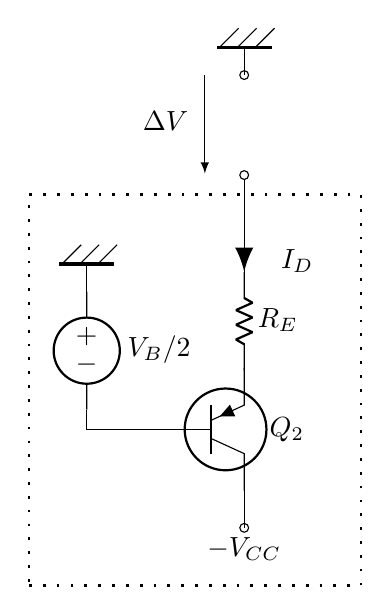
\begin{tikzpicture}
	\node[shape=rectangle, draw, line width=1pt, dash pattern={on 1pt off 4pt}, minimum width=4.215cm, minimum height=4.965cm] at (2.375, 2.5){};
	\draw[-latex] (2.5, 6.5) -- (2.5, 5.25);
	\node[shape=rectangle, minimum width=1.215cm, minimum height=0.715cm] at (2, 5.875){} node[anchor=north, align=center, text width=0.827cm, inner sep=6pt] at (2, 6.25){$\Delta V$};
	\node[pnp, tr circle](N1) at (3, 2){} node[anchor=west] at ([xshift=0.13cm]N1.text){$Q_2$};
	\draw (3, 4) to[american resistor, /tikz/circuitikz/bipoles/length=0.700cm, l={$R_E$}] (3, 2.75);
	\draw (3, 5.23) -- (3, 4);
	\draw[line width=2pt, -latex] (3, 4.25) -- (3, 4);
	\node[ocirc](N2) at (3, 0.75){} node[anchor=north] at (N2.text){$-V_{CC}$};
	\draw (3, 0.75) -- (3, 1.23);
	\node[ocirc] at (3, 5.23){};
	\node[ocirc] at (3, 6.5){};
	\draw (1, 3.75) to[american voltage source, l={$V_B/2$}] (1, 2.25);
	\draw (2.16, 2) -| (1, 2.25);
	\node[eground2, xscale=-1, yscale=-1] at (1, 3.75){};
	\node[eground2, xscale=-1, yscale=-1] at (3, 6.5){};
	\node[shape=rectangle, minimum width=0.965cm, minimum height=0.715cm] at (3.75, 4.125){} node[anchor=north west, align=left, text width=0.577cm, inner sep=6pt] at (3.25, 4.5){$I_D$};
\end{tikzpicture}

The equation looks like the one we got for the current source version:
$$
I_D = f_D \left(\Delta V + \dfrac{v_B}{2} - R_E I_D \right) \\
$$

And:
\fbox{$I_D = \dfrac{1}{R_E}\dfrac{a R_E}{1+a R_E}\Delta V + \dfrac{a \frac{V_B}{2} + b}{1 + a R_E} = \hat{f}_D (\Delta V)$}

\subsection*{Class AB subsystem: summary}
Let's see now how we can combine the subsystems to solve for the class AB entirely. Recall the simplified view of the system:


\begin{circuitikz}
	\draw (1, 5) -| (2, 5);
	\draw (4, 4.25) -- (4, 5.75);
	\draw (2, 5.75) -| (2, 4.25);
	\draw (4, 5) -| (5.75, 4.75);
	\draw (5.75, 4.75) to[american resistor, /tikz/circuitikz/bipoles/length=0.700cm, l={$R_L$}] (5.75, 3.5);
	\node[circ] at (4, 5){};
	\node[eground2] at (5.75, 3.5){};
	\node[circ] at (2, 5){};
	\node[ocirc](N1) at (1, 5){} node[anchor=east] at (N1.text){$V_{IN}$};
	\draw[-latex] (6.75, 3.5) -- (6.75, 4.75);
	\node[shape=rectangle, minimum width=0.965cm, minimum height=0.715cm] at (7.25, 4.125){} node[anchor=north west, align=left, text width=0.577cm, inner sep=6pt] at (6.75, 4.5){$V_{OUT}$};
	\draw[dash pattern={on 0.4pt off 1.6pt}] (5.75, 5) -- (7, 5);
	\node[shape=rectangle, draw, line width=1pt, minimum width=2.965cm, minimum height=1.465cm] at (3, 6.5){} node[anchor=center, align=center, text width=2.577cm, inner sep=6pt] at (3, 6.5){Source subsystem};
	\node[shape=rectangle, draw, line width=1pt, minimum width=2.965cm, minimum height=1.465cm] at (3, 3.5){} node[anchor=center, align=center, text width=2.577cm, inner sep=6pt] at (3, 3.5){Drain subsystem};
	\draw[line width=1pt, -latex] (2.25, 5) -- (3.75, 5);
	\node[shape=rectangle, minimum width=0.965cm, minimum height=0.715cm] at (3, 4.625){} node[anchor=north west, align=left, text width=0.577cm, inner sep=6pt] at (2.5, 5){$\Delta V$};
	\draw[line width=1.5pt, -latex] (4, 5.5) -| (4, 5.25);
	\draw[line width=1.5pt, -latex] (4, 4.75) -| (4, 4.5);
	\node[shape=rectangle, minimum width=0.965cm, minimum height=0.715cm] at (4.5, 5.375){} node[anchor=north west, align=left, text width=0.577cm, inner sep=6pt] at (4, 5.75){$I_S$};
	\node[shape=rectangle, minimum width=0.965cm, minimum height=0.715cm] at (4.5, 4.625){} node[anchor=north west, align=left, text width=0.577cm, inner sep=6pt] at (4, 5){$I_D$};
	\draw[line width=1.5pt, -latex] (5.25, 5) -- (5.5, 5);
	\node[shape=rectangle, minimum width=0.965cm, minimum height=0.715cm] at (5.5, 5.375){} node[anchor=north west, align=left, text width=0.577cm, inner sep=6pt] at (5, 5.75){$I_L$};
\end{circuitikz}

Therefore:\\

$$
	V_{OUT} = R_L \left( \hat{f}_S \left(V_{IN} - V_{OUT} \right) - \hat{f}_D \left(V_{OUT} - V_{IN} \right) \right)
$$\\

The equation exhibits an ultimate recursion that we need to get rid of. For that, we need to study this last function:
$$
	\hat{f}(\Delta V) \triangleq \hat{f}_S(-\Delta V) - \hat{f}_D(\Delta V)
$$

To simplify the analysis, we consider that $\Delta V^F = 0$.


By linearity, we know that $\hat{f}$ is piecewise linear too.



Then:
$$
	V_{OUT} = R_L\hat{f}(V_{OUT}-V_{IN}) 
$$
This looks familiar: it is the equation for the emitter follower!


\subsection*{Conclusions}

\begin{itemize}
	\item No need for strong matching between the transistors
	\item Role of $R_E$
	\item What if $\Delta V^F \neq 0$?
\end{itemize}



\section*{Example 7: the Differential Pair}

The Differential Pair (or Long Tailed Pair ¬‿¬) is the core element of Operational Amplifiers. It is a voltage difference amplifier achieving very high gain and you'd meet this structure in schematics until the eighties, when the price of op amps eventually decreased and their performance beat the discrete version.

\begin{circuitikz}
	\node[npn, tr circle](N1) at (5.84, 10){} node[anchor=west] at ([xshift=0.08cm]N1.text){$Q_1$};
	\node[npn, tr circle, xscale=-1](N2) at (8.16, 10){} node[anchor=east] at ([xshift=-0.08cm]N2.text){$Q_2$};
	\draw (5.84, 9.23) to[american resistor, /tikz/circuitikz/bipoles/length=0.700cm, l={$R_E$}] (5.84, 7.98);
	\draw (8.16, 9.23) to[american resistor, /tikz/circuitikz/bipoles/length=0.700cm, l={$R_E$}] (8.16, 7.98);
	\draw (5.84, 12.02) to[american resistor, /tikz/circuitikz/bipoles/length=0.700cm, l={$R_C$}] (5.84, 10.77);
	\draw (8.16, 12.02) to[american resistor, /tikz/circuitikz/bipoles/length=0.700cm, l={$R_C$}] (8.16, 10.77);
	\draw (9, 10) -| (9.25, 10);
	\draw (4.75, 10) -| (5, 10);
	\draw (5.84, 7.98) |- (6.25, 7.5) -| (8.16, 7.98);
	\draw (5.84, 12.02) |- (6, 12.5) -| (8.16, 12.02);
	\node[vcc] at (7, 13){};
	\draw (7, 13) -| (7, 12.5);
	\node[circ] at (7, 12.5){};
	\draw (7, 7) to[oosourcetrans] (7, 5.25);
	\node[eground2] at (7, 5.25){};
	\node[circ] at (7, 7.5){};
	\draw (9.25, 10) to[american resistor, /tikz/circuitikz/bipoles/length=0.700cm, l={$R_B$}] (10.25, 10);
	\draw (10.25, 10) -- (10.5, 10);
	\node[ocirc](N3) at (10.5, 10){} node[anchor=west] at ([xshift=0.08cm]N3.text){$V_{M}$};
	\draw (3.75, 10) to[american resistor, /tikz/circuitikz/bipoles/length=0.700cm, l={$R_B$}] (4.75, 10);
	\draw (3.5, 10) -- (3.75, 10);
	\node[ocirc](N4) at (3.5, 10){} node[anchor=east] at ([xshift=-0.08cm]N4.text){$V_{P}$};
	\draw (7, 7) -| (7, 7.5);
	\draw[line width=2pt, -latex] (7, 7) -- (7, 6.75);
	\draw[line width=2pt, -latex] (5.84, 12.02) -- (5.84, 11.77);
	\draw[line width=2pt, -latex] (8.16, 12.02) -- (8.16, 11.77);
	\node[shape=rectangle, minimum width=0.715cm, minimum height=0.715cm](N5) at (7.375, 6.875){} node[anchor=center] at (N5.text){$I$};
	\node[shape=rectangle, minimum width=0.715cm, minimum height=0.715cm](N6) at (5.375, 12){} node[anchor=center] at (N6.text){$I_P$};
	\node[shape=rectangle, minimum width=0.715cm, minimum height=0.715cm](N7) at (8.625, 12){} node[anchor=center] at (N7.text){$I_M$};
\end{circuitikz}

We consider the most general case with emitter and base resistors. Adding the base resistors $R_B$ will help later on to study the offset compensation. The emitter degeneration resistors $R_E$ are the most interesting part as they are responsible for making the analysis particularly difficult in the general case (no closed-form solution).

The voltage equation yields:
$$
	\left(R_E + \dfrac{R_B}{\beta} \right)I_P
$$\\


\section*{Example 8: the \textit{Ring Modulator}}

The Ring Modulator is a special arrangement of diodes that, under certain conditions, produces a voltage that is the mathematical product of 2 input voltages. The term \textit{modulator} comes from the fact that this was the way radio-electric modulation was achieved back in the days. This diode structure appeared in patents dating back from 1934\footnote{US Patent 2,025,158 \textit{Modulating System}, F. A. Cowan, 24 Dec 1934} (!). 

Notice how the structure slightly differs from the good old Full Bridge Rectifier (or \textit{Graetz Bridge}). Though the Bridge Rectifier has other aces up its sleeves, as we will see in the next section.

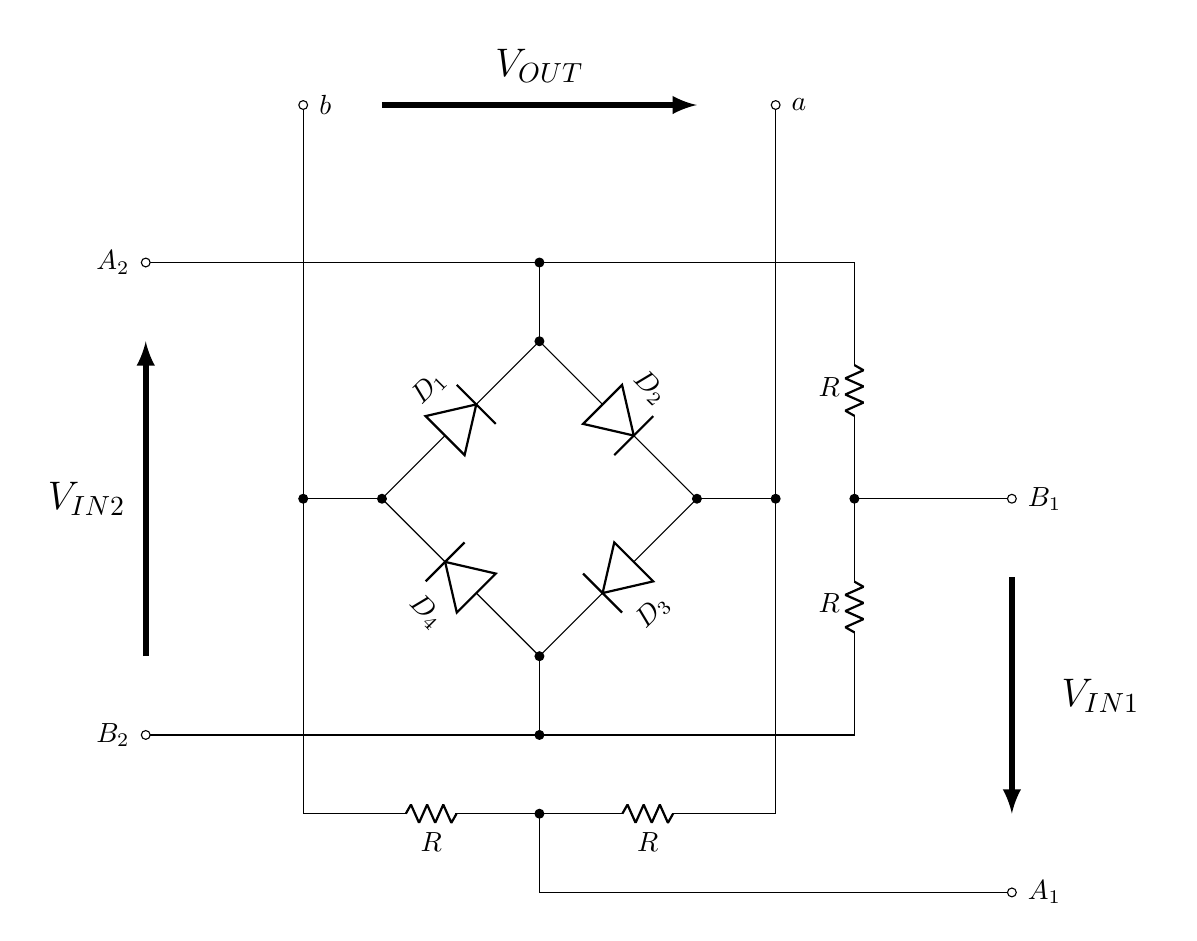
\begin{tikzpicture}
	\draw (9.75, -0) to[american resistor, /tikz/circuitikz/bipoles/length=0.770cm, l={$R$}] (7.5, -0);
	\draw (10, 6) to[empty diode, l={$D_2$}] (12, 4);
	\node[circ] at (8, 4){};
	\draw (12, 4) to[empty diode, l={$D_3$}] (10, 2);
	\draw (10, 2) to[empty diode, l={$D_4$}] (8, 4);
	\draw (8, 4) to[empty diode, l={$D_1$}] (10, 6);
	\node[circ] at (12, 4){};
	\node[circ] at (10, 6){};
	\node[circ] at (10, 2){};
	\draw (12.5, -0) to[american resistor, /tikz/circuitikz/bipoles/length=0.770cm, l={$R$}] (10.25, -0);
	\draw (12.5, -0) -| (13, 4) -- (12, 4);
	\draw (14, 4.25) to[american resistor, /tikz/circuitikz/bipoles/length=0.770cm, l={$R$}] (14, 6.5);
	\draw (14, 1.5) to[american resistor, /tikz/circuitikz/bipoles/length=0.770cm, l={$R$}] (14, 3.75);
	\draw (14, 1.5) |- (10, 1) -- (10, 2);
	\draw (7.5, -0) -| (7, 4) -- (8, 4);
	\draw (14, 6.5) -- (14, 7) -- (10, 7) -- (10, 6);
	\draw (9.75, -0) -- (10.25, -0);
	\draw (14, 3.75) -| (14, 4.25);
	\draw (14, 4) -- (16, 4);
	\node[circ] at (14, 4){};
	\draw (10, 7) -- (5, 7);
	\node[circ] at (10, 7){};
	\node[circ] at (10, -0){};
	\node[circ] at (10, 1){};
	\draw (5, 1) -- (10, 1);
	\draw (16, -1) -| (10, -0);
	\draw (13, 4) |- (13, 9);
	\draw (7, 4) -- (7, 9);
	\node[ocirc](N1) at (13, 9){} node[anchor=west] at ([xshift=0.08cm]N1.text){$a$};
	\node[ocirc](N2) at (7, 9){} node[anchor=west] at ([xshift=0.08cm]N2.text){$b$};
	\node[circ] at (7, 4){};
	\node[circ] at (13, 4){};
	\draw[line width=2pt, -latex] (5, 2) -- (5, 6);
	\draw[line width=2pt, -latex] (16, 3) -- (16, -0);
	\draw[line width=2pt, -latex] (8, 9) -- (12, 9);
	\node[shape=rectangle, minimum width=3.965cm, minimum height=0.965cm] at (10, 9.5){} node[anchor=center, align=center, text width=3.577cm, inner sep=6pt] at (10, 9.5){\Large $V_{OUT}$};
	\node[shape=rectangle, minimum width=1.465cm, minimum height=3.965cm] at (4.25, 4){} node[anchor=center, align=center, text width=1.077cm, inner sep=6pt] at (4.25, 4){\Large $V_{IN 2}$};
	\node[shape=rectangle, minimum width=1.715cm, minimum height=2.965cm] at (17.125, 1.5){} node[anchor=center, align=center, text width=1.327cm, inner sep=6pt] at (17.125, 1.5){\Large $V_{IN1}$};
	\node[ocirc](N3) at (5, 7){} node[anchor=east] at ([xshift=-0.08cm]N3.text){$A_2$};
	\node[ocirc](N4) at (5, 1){} node[anchor=east] at ([xshift=-0.08cm]N4.text){$B_2$};
	\node[ocirc](N5) at (16, 4){} node[anchor=west] at ([xshift=0.08cm]N5.text){$B_1$};
	\node[ocirc](N6) at (16, -1){} node[anchor=west] at ([xshift=0.08cm]N6.text){$A_1$};
\end{tikzpicture}

At first glance, the wizardry by which this achieves multiplication is not obvious.

*** SECTION IS TODO ***



\section*{Example 9: the Bridge Rectifier as variable resistor}

This time, we will study how an actual diode bridge (the same as the one you'd use to rectify AC) can be used as a variable resistor. There are patented references to that in 1971\footnote{US Patent 3,582,807 \textit{Amplifier Gain Control Circuit Including Diode Bridge}, John L. Addis, 1st June 1971} and 1975\footnote{US Patent 4,039,980 \textit{Voltage Controlled Filter}, Yasuo Nagahama, 29 July 1975} with a direct application to Voltage-Controlled Filters.





\section*{Example 10: the Gilbert Cell (analog multiplier)}
That's a tough one, be patient...




\section*{Example 11: the Moog Ladder Filter}

\subsubsection*{Description}
The Moog Ladder Filter is a parametric low-pass filter used in analog synthesizers.\\

Its cutoff frequency can be freely adjusted using a control current, which makes it a very unique kind of filter.
It gained its popularity and fame in the Moog Synthesizers, as early as the seventies. 
The term \textit{Ladder Filter} comes from the way the schematic looks: its very much \textit{ladder-like}. 

The full circuit might look intimidating at first. Let's zoom in on its building block:

\begin{circuitikz}
	\draw (3, 3.98) -- (3, -0.23);
	\draw[line width=2pt, -latex] (3, 0.02) -- (3, -0.23);
	\node[shape=rectangle, minimum width=1.965cm, minimum height=0.985cm] at (1.75, 0.03){} node[anchor=north east, align=right, text width=1.577cm, inner sep=6pt] at (2.75, 0.54){$I_C - \dfrac{\Delta I}{2}$};
	\node[npn, tr circle](N1) at (5.5, 4.75){} node[anchor=west] at ([xshift=0.13cm]N1.text){$Q_2$};
	\node[npn, tr circle, xscale=-1](N2) at (3, 4.75){} node[anchor=east] at ([xshift=-0.13cm]N2.text){$Q_1$};
	\draw (0.5, 5.75) -| (4.25, 4.75);
	\draw[dash pattern={on 1.6pt off 1.6pt}] (3, -1.73) -- (3, -2.5);
	\draw (5.5, 3.98) -- (5.5, -0.25);
	\draw (3, 3.25) -- (8, 3.25);
	\draw (3.84, 4.75) -- (4.66, 4.75);
	\draw[line width=2pt, -latex] (7.25, 3.25) -- (7.5, 3.25);
	\node[shape=rectangle, minimum width=2.215cm, minimum height=0.985cm] at (6.875, -0.01){} node[anchor=north west, align=left, text width=1.827cm, inner sep=6pt] at (5.75, 0.5){$I_C + \dfrac{\Delta I}{2}$};
	\node[circ] at (3, 3.25){};
	\node[circ] at (5.5, 1.75){};
	\draw (3, -0.23) to[ioosource] (3, -1.73);
	\draw (5.5, -0.25) to[ioosource] (5.5, -1.75);
	\node[ocirc](N3) at (8, 3.25){} node[anchor=west] at (N3.east){$V_P$};
	\draw[dash pattern={on 1.6pt off 1.6pt}] (5.5, -1.75) -- (5.5, -2.52);
	\draw[line width=2pt, -latex] (9.375, 2) -- (9.375, 3);
	\node[shape=rectangle, minimum width=0.715cm, minimum height=1.465cm] at (10, 2.5){} node[anchor=center, align=center, text width=0.327cm, inner sep=6pt] at (10, 2.5){$\Delta V$};
	\node[circ] at (4.25, 4.75){};
	\draw (5.5, 1.75) -| (8, 1.75);
	\node[ocirc](N4) at (8, 1.75){} node[anchor=west] at (N4.east){$V_M$};
	\node[ocirc](N5) at (0.5, 5.75){} node[anchor=east] at (N5.west){$V_{BIAS}$};
	\draw[line width=2pt, -latex] (7.5, 1.75) -- (7.221, 1.75);
	\draw[line width=2pt, -latex] (5.5, -0) -- (5.5, -0.25);
	\node[shape=rectangle, minimum width=0.686cm, minimum height=0.465cm] at (7.36, 3.75){} node[anchor=west, align=left, text width=0.297cm, inner sep=6pt] at (7, 3.75){$I_P$};
	\node[shape=rectangle, minimum width=0.686cm, minimum height=0.465cm] at (7.36, 2.25){} node[anchor=west, align=left, text width=0.297cm, inner sep=6pt] at (7, 2.25){$I_M$};
	\draw[dash pattern={on 0.4pt off 1.6pt}] (8.875, 3.25) -- (10.375, 3.25);
	\draw[dash pattern={on 0.4pt off 1.6pt}] (8.875, 1.75) -- (10.375, 1.75);
	\draw[dash pattern={on 1.6pt off 1.6pt}] (5.5, 8.5) -- (5.5, 7.5);
	\draw[dash pattern={on 1.6pt off 1.6pt}] (3, 8.5) -- (3, 7.5);
	\draw (3, 5.52) |- (3, 7.5);
	\draw (5.5, 7.5) |- (5.5, 5.52);
	\draw[line width=2pt, -latex] (3, 7.25) -- (3, 7);
	\draw[line width=2pt, -latex] (5.5, 7.25) -- (5.5, 7);
	\node[shape=rectangle, minimum width=2.215cm, minimum height=0.985cm] at (6.875, 7.25){} node[anchor=north west, align=left, text width=1.827cm, inner sep=6pt] at (5.75, 7.76){$I_C + \dfrac{\Delta I'}{2}$};
	\node[shape=rectangle, minimum width=1.965cm, minimum height=0.985cm] at (1.75, 7.26){} node[anchor=north east, align=right, text width=1.577cm, inner sep=6pt] at (2.75, 7.77){$I_C - \dfrac{\Delta I'}{2}$};
	\node[shape=rectangle, draw, line width=1pt, dash pattern={on 4pt off 4pt}, minimum width=4.965cm, minimum height=4.985cm] at (4.25, 3.74){};
\end{circuitikz}

This building block can be seen as a \textbf{current transformation} core. A balanced current is drawn from the bottom section, and another pair of currents emerges from the top section. 

The bottom currents are imposed. We don't know the top currents yet, but considering the symmetry of the circuit, it makes sense to denote them as a differential mode current too: $I_C \pm \frac{\Delta I'}{2}$.\\

The current drawn from the bottom of the block has specific properties:
\begin{itemize}
	\item A \textbf{control} current $I_C$ applied in common mode
	\item A \textbf{signal} current $\frac{\Delta I}{2}$ applied in differential mode.
\end{itemize}
Such source is straightforward with the Differential Pair studied earlier.\\

Let's analyse how the circuit behaves as we load it:
\begin{itemize}
	\item $I_P = I_M \triangleq I$
	\item $V_P - V_M \triangleq \Delta V$.
\end{itemize}

If we denote $(I, i)$ as a current pair of common mode current $I$ and differential mode $i/2$, the schematic can be further simplified to:

\begin{circuitikz}
	\node[shape=rectangle, minimum width=3.465cm, minimum height=0.965cm] at (4.25, 1.25){} node[anchor=center, align=center, text width=3.077cm, inner sep=6pt] at (4.25, 1.25){$(I_C, \Delta I)$};
	\node[shape=rectangle, minimum width=3.465cm, minimum height=0.965cm] at (4.25, 6.75){} node[anchor=center, align=center, text width=3.077cm, inner sep=6pt] at (4.25, 6.75){$(I_C, \Delta I')$};
	\node[shape=rectangle, draw, line width=1pt, dash pattern={on 4pt off 4pt}, minimum width=4.965cm, minimum height=4.465cm] at (4.25, 4){};
	\draw (3, 3.98) -- (3, 1);
	\draw[line width=2pt, -latex] (3, 1.5) -- (3, 1.25);
	\node[npn, tr circle](N1) at (5.5, 4.75){} node[anchor=west] at ([xshift=0.13cm]N1.text){$Q_2$};
	\node[npn, tr circle, xscale=-1](N2) at (3, 4.75){} node[anchor=east] at ([xshift=-0.13cm]N2.text){$Q_1$};
	\draw (0.5, 5.75) -| (4.25, 4.75);
	\draw[dash pattern={on 1.6pt off 1.6pt}] (3, -0.48) -- (3, -1.25);
	\draw (5.5, 3.98) -- (5.5, 1);
	\draw (3, 3.25) -- (3.5, 3.25);
	\draw (3.84, 4.75) -- (4.66, 4.75);
	\draw[line width=2pt, -latex] (3.25, 3.25) -- (3.5, 3.25);
	\node[circ] at (3, 3.25){};
	\node[circ] at (5.5, 3.25){};
	\draw (3, 1) to[ioosource] (3, -0.5);
	\draw (5.5, 1) to[ioosource] (5.5, -0.5);
	\draw[dash pattern={on 1.6pt off 1.6pt}] (5.5, -0.5) -- (5.5, -1.27);
	\draw[line width=2pt, -latex] (5, 2.75) -- (3.5, 2.75);
	\node[shape=rectangle, minimum width=0.715cm, minimum height=1.465cm] at (4.25, 2.25){} node[anchor=center, align=center, text width=0.327cm, inner sep=6pt] at (4.25, 2.25){$\Delta V$};
	\node[circ] at (4.25, 4.75){};
	\draw (5.5, 3.25) -- (5, 3.25);
	\node[ocirc](N3) at (0.5, 5.75){} node[anchor=east] at (N3.west){$V_{BIAS}$};
	\node[shape=rectangle, minimum width=0.686cm, minimum height=0.465cm] at (3.36, 3.73){} node[anchor=west, align=left, text width=0.297cm, inner sep=6pt] at (3, 3.73){$I$};
	\draw[dash pattern={on 1.6pt off 1.6pt}] (5.5, 8.25) -- (5.5, 7.25);
	\draw[dash pattern={on 1.6pt off 1.6pt}] (3, 8.25) -- (3, 7.25);
	\draw (3, 5.52) |- (3, 7.25);
	\draw (5.5, 7.25) |- (5.5, 5.52);
	\draw[line width=2pt, -latex] (3, 6.75) -- (3, 6.5);
	\draw[line width=2pt, -latex] (5.5, 6.75) -- (5.5, 6.5);
	\draw (3.5, 3.25) to[european resistor, /tikz/circuitikz/bipoles/length=1.05cm, l={$Z$}] (5, 3.25);
	\draw[line width=2pt, -latex] (5.5, 1.5) -- (5.5, 1.25);
\end{circuitikz}

Now the questions are essentially: 
\begin{itemize}
	\item What is the differential current transfer function $\Delta I' = H(\Delta I)$?
	\item What is voltage transfer function $\Delta V = G(\Delta I)$?
\end{itemize}

\subsection*{Output Voltage derivation}
As usual we denote the collector current $I_C$ as $I_C = f(V_{BE})$. We neglect the contribution of the base current and assume the transistors have similar properties.

With KCL we get:
$$
\left\{
	\begin{array}{ll}
		I_P = f(V_{BIAS}-V_P) - I_C + \dfrac{\Delta I}{2}\\
		I_M = -f(V_{BIAS}-V_M) + I_C + \dfrac{\Delta I}{2}
	\end{array}
\right.
$$

With the piecewise linear assumption it becomes:
$$
\left\{
	\begin{array}{ll}
		I_P = -a V_P - I_C + \dfrac{\Delta I}{2} + a V_{BIAS} + b\\
		I_M = a V_M + I_C + \dfrac{\Delta I}{2} - a V_{BIAS} - b
	\end{array}
\right.
$$

Once loaded, summing the 2 equations gives:
$$
2I = -a \Delta V + \Delta I
$$

If the load is a simple impedance $Z$, then $I = \frac{\Delta V}{Z}$. Also, remember that $a$ is the gain in the $I_C = f(V_{BE})$ relationship, therefore it can be seen as an inverse resistance (the \textit{dynamic} resistance).

So we can write $a \triangleq \frac{1}{R_C}$, we get this rather \textit{nice} expression:
$$
\Delta V = \left[ \dfrac{(2R_C) Z}{(2R_C) + Z} \right] \dfrac{\Delta I}{2}
$$

Which is also known as:
$$
\Delta V = \left( 2R_C // Z \right) \dfrac{\Delta I}{2}
$$

This is an elementary $V=RI$ relationship!\\

So from the load's perspective, it's as if it were stimulated with the signal (differential current $\Delta I$), parallel to some resistance $2R_C$ that depends on the transconductance of $Q1$ and $Q2$ (\textit{i.e.} the gain $a$ in the piecewise linear model).


\begin{circuitikz}
	\draw (1.75, 3.25) -| (1.75, 4.5);
	\draw[line width=2pt, -latex] (1.75, 4.04) -| (1.75, 3.75);
	\draw[dash pattern={on 1.6pt off 1.6pt}] (4.5, 3.25) -- (2.75, 3.25);
	\draw[line width=2pt, -latex] (3.625, 1.25) -- (3.625, 3);
	\node[shape=rectangle, minimum width=0.715cm, minimum height=1.715cm] at (4, 2.125){} node[anchor=center, align=center, text width=0.327cm, inner sep=6pt] at (4, 2.125){$\Delta V$};
	\draw (2.5, 3) to[european resistor, /tikz/circuitikz/bipoles/length=1.05cm, l={$Z$}] (2.5, 1.25);
	\draw (1, 2.75) to[american resistor, /tikz/circuitikz/bipoles/length=0.700cm, l_={$2R_C$}] (1, 1.5);
	\draw (1, 1.5) -- (1, 1) -- (2.5, 1) -| (2.5, 1.25);
	\draw (1, 2.75) -- (1, 3.25) -| (2.5, 3);
	\node[circ] at (1.75, 3.25){};
	\node[circ] at (1.75, 1){};
	\draw[dash pattern={on 1.6pt off 1.6pt}] (4.5, 1) -| (2.75, 1);
	\draw (1.75, 1) -- (1.75, 0.5);
	\node[shape=rectangle, minimum width=1.075cm, minimum height=0.965cm] at (2.445, 4){} node[anchor=west, align=left, text width=0.687cm, inner sep=6pt] at (1.89, 4){$\dfrac{\Delta I}{2}$};
	\draw[dash pattern={on 1.6pt off 1.6pt}] (1.75, -0) -| (1.75, 0.5);
	\draw[dash pattern={on 1.6pt off 1.6pt}] (1.75, 4.5) -| (1.75, 5.25);
\end{circuitikz}


\subsubsection*{Comparison without active loading}
To fully understand this result, we now study what would happen without the transistors.


%\subsubsection*{The Resistive load case}
%With $Z=R$ we simply get:
%$$
%\Delta V = -\dfrac{1}{2} \left[ \dfrac{(2R_C) R}{(2R_C) + R} \right] \Delta I
%$$\\
%
%
%
%From the output perspective, we see a parallel resistor association: $2R_C$ and $R$, with some gain $-1/2$.
%
%\subsubsection*{The Capacitive load case}
%For a capacitive load, $Z = \frac{1}{jC\omega}$. We write $a = \frac{1}{R}$ thus:
%
%\fbox{$\Delta V = R\dfrac{-1}{1 + 2jRC\omega} \Delta I$}
%
%
%Now the key element to understand how this can be a parametric filter is to go back to the definition of $a$: $a$ is a function of the control current $I_C$.
%
%In the previous examples we didn't care much about the transconductance $a$.


\subsection*{Output current derivation}
We've established that:
$$
\left\{
	\begin{array}{ll}
		I_P = f(V_{BIAS}-V_P) - I_C + \dfrac{\Delta I}{2}\\
		I_M = -f(V_{BIAS}-V_M) + I_C + \dfrac{\Delta I}{2}
	\end{array}
\right.
$$

The output current $\Delta I'$ is defined by :
$$
\left\{
	\begin{array}{ll}
		I_C - \dfrac{\Delta I'}{2} = f(V_{BIAS} - V_P)\\
		I_C + \dfrac{\Delta I'}{2} = f(V_{BIAS} - V_M)
	\end{array}
\right.
$$

Combining the 2 systems of equations we get:
$$
\left\{
	\begin{array}{ll}
		\dfrac{\Delta I'}{2} = \dfrac{\Delta I}{2} - I_P\\
		\dfrac{\Delta I'}{2} = \dfrac{\Delta I}{2} - I_M
	\end{array}
\right.
$$

Summing the 2 finally gives:
\fbox{$\Delta I' = \Delta I  - 2I$}\\

With a load impedance $Z$ it follows that:
\begin{equation}
\begin{split}
\Delta I'	& = \Delta I - \dfrac{2}{Z} \Delta V \\
 			& = \Delta I - \dfrac{2}{Z} (2R_C // Z) \dfrac{\Delta I}{2}\\
			& = \left( 1 - \dfrac{2R_C}{2R_C + Z} \right) \Delta I\\
			& = \dfrac{Z}{2R_C + Z} \Delta I
\end{split}
\end{equation}

So finally the differential current transfer function:
\fbox{$\Delta I' = \dfrac{Z}{2R_C + Z} \Delta I$}\\

We can update the abstract schematic view in terms of \textit{current transformation}:

\begin{circuitikz}
	\node[shape=rectangle, minimum width=3.465cm, minimum height=0.965cm] at (4.25, 3.27){} node[anchor=center, align=center, text width=3.077cm, inner sep=6pt] at (4.25, 3.27){$(I_C, \Delta I)$};
	\node[shape=rectangle, minimum width=3.465cm, minimum height=0.965cm] at (4.25, 6.75){} node[anchor=center, align=center, text width=3.077cm, inner sep=6pt] at (4.25, 6.75){$(I_C, \dfrac{Z}{2R_C + Z} \Delta I)$};
	\node[shape=rectangle, draw, line width=1pt, dash pattern={on 4pt off 4pt}, minimum width=4.965cm, minimum height=1.715cm] at (4.25, 4.875){};
	\draw (2.25, 4.25) -| (2.25, 2.25);
	\draw[line width=2pt, -latex] (2.25, 2.75) -- (2.25, 2.5);
	\draw[dash pattern={on 1.6pt off 1.6pt}] (2.25, 0.77) -- (2.25, -0);
	\draw (6.25, 4.27) -| (6.25, 2.27);
	\draw (2.25, 2.25) to[ioosource] (2.25, 0.75);
	\draw (6.25, 2.27) to[ioosource] (6.25, 0.77);
	\draw[dash pattern={on 1.6pt off 1.6pt}] (6.25, 0.77) -- (6.25, -0);
	\draw[dash pattern={on 1.6pt off 1.6pt}] (6.25, 8.23) -- (6.25, 7.23);
	\draw[dash pattern={on 1.6pt off 1.6pt}] (2.25, 8.23) -- (2.25, 7.23);
	\draw (2.25, 5.5) -- (2.25, 7.23);
	\draw (6.25, 7.23) -- (6.25, 5.5);
	\draw[line width=2pt, -latex] (2.25, 6.73) -- (2.25, 6.48);
	\draw[line width=2pt, -latex] (6.25, 6.73) -- (6.25, 6.48);
	\draw (3.5, 4.75) to[european resistor, /tikz/circuitikz/bipoles/length=1.05cm, l={$Z$}] (5, 4.75);
	\draw[line width=2pt, -latex] (6.25, 2.77) -- (6.25, 2.52);
\end{circuitikz}


From which we can derive 2 regimes:
\begin{itemize}	
	\item $R_C \gg \left|Z\right|$ (low $I_C$): $\Delta I \rightarrow 0$
	\item $R_C \ll \left|Z\right|$ (high $I_C$): $\Delta I \rightarrow \Delta I$ (no change)
\end{itemize}


Let's get more precise. The dynamic resistance (so the gain in the I/V curve) $R_C$ can be expressed explicitly as a function of $I_C$ therefore giving a more refined description of the transfer curve.

For a BJT:
\begin{equation}
\begin{split}
	a	& = \left. \frac{\partial I_C}{\partial V_{BE}} \right|_{V_{BE} = V_{BE}^0}\\
 		& = \left. \frac{\partial }{\partial V_{BE}} \right|_{V_{BE} = V_{BE}^0} I_S \exp \left( \right)\\
		& = \left( 1 - \dfrac{2R_C}{2R_C + Z} \right) \Delta I\\
		& = \dfrac{Z}{2R_C + Z} \Delta I
\end{split}
	a = 
\end{equation}

 
\subsection*{Limits}


\subsubsection*{Large signal analysis}
Unlike the Emitter Follower, there's no feedback here to rely on. Hence, we expect deviation from the model if the input is too wide.

\subsubsection*{Transistor spec mismatch}
This section is TODO.



\section*{Example 12: the diode Ladder Filter}

\subsubsection*{Description}
As a follow-up of the Moog Ladder Filter, we now consider the case of the diode version. It looks very similar to the Moog one, except the BJTs have been replaced with diodes. 



\section*{Example 13: the Moog Voltage Controlled High-Pass filter (module \textit{904B})}

\subsubsection*{Description}
Similarly, Moog came up with a design for a high-pass filter (also patented). The structure differs a bit from the low-pass, but it is equally as puzzling.

Here below is one stage of the high-pass filter:

\begin{circuitikz}
\node[npn, tr circle](N1) at (6, 4.02){} node[anchor=west] at ([xshift=0.13cm]N1.text){$Q_1$};
	\node[npn, tr circle](N2) at (9.5, 2.75){} node[anchor=west] at ([xshift=0.13cm]N2.text){$Q_3$};
	\node[pnp, tr circle](N3) at (6, 1.48){} node[anchor=west] at ([xshift=0.13cm]N3.text){$Q_2$};
	\draw (6, 2.25) -- (6, 3.25);
	\node[circ] at (6, 2.75){};
	\draw (4.5, 4.75) |- (5.16, 4.02);
	\node[ocirc](N4) at (4.5, 4.75){} node[anchor=south] at ([yshift=0.13cm]N4.north){$E$};
	\draw (4.5, 0.75) |- (5.16, 1.48);
	\node[ocirc](N5) at (4.5, 0.75){} node[anchor=north] at ([yshift=-0.13cm]N5.text){$-E$};
	\draw (6, 7.25) to[american resistor, /tikz/circuitikz/bipoles/length=0.700cm, l={$R_1$}, label distance=0.13cm] (6, 5.75);
	\draw (6, 5.75) -| (6, 4.79);
	\draw (6, -0.25) to[american resistor, /tikz/circuitikz/bipoles/length=0.700cm, l={$R_2$}, label distance=0.13cm] (6, -1.75);
	\draw (6, -0.25) -| (6, 0.71);
	\draw (3.75, 2.75) to[capacitor, /tikz/circuitikz/bipoles/length=0.700cm] (2.25, 2.75);
	\node[ocirc](N6) at (6, 7.25){} node[anchor=south] at ([yshift=0.13cm]N6.north){$V_{CC}$};
	\node[ocirc](N7) at (6, -1.75){} node[anchor=north] at ([yshift=-0.13cm]N7.text){$-V_{CC}$};
	\draw (3.75, 2.75) -- (6, 2.75);
	\node[pnp, tr circle](N8) at (10.75, 4.008){} node[anchor=west] at ([xshift=0.13cm]N8.text){$Q_4$};
	\draw (9.5, 7.25) to[american resistor, /tikz/circuitikz/bipoles/length=0.700cm, l_={$R_3$}, label distance=0.13cm] (9.5, 5.75);
	\node[ocirc](N9) at (9.5, 7.25){} node[anchor=south] at ([yshift=0.13cm]N9.north){$V_{CC}$};
	\draw (6, 2.75) -| (8.66, 2.75);
	\draw (9.5, 3.52) -| (9.5, 5.75);
	\draw (10.75, 4.79) -| (10.75, 5.29);
	\node[ocirc](N10) at (10.75, 5.29){} node[anchor=south] at ([yshift=0.13cm]N10.north){$V_{POL}$};
	\draw (9.5, 2) |- (12, 1.5);
	\draw (10.75, 3.25) -- (10.75, 1.5);
	\draw (9.91, 4.008) -| (9.5, 3.988);
	\draw (9.5, -0.25) to[american resistor, /tikz/circuitikz/bipoles/length=0.700cm, l_={$R_4$}, label distance=0.13cm] (9.5, -1.75);
	\node[ocirc](N11) at (9.5, -1.75){} node[anchor=north] at ([yshift=-0.13cm]N11.text){$-V_{CC}$};
	\draw (9.5, -0.25) -| (9.5, 1.5);
	\node[circ] at (9.5, 1.5){};
	\node[circ] at (10.75, 1.5){};
	\node[circ] at (9.5, 4){};
	\node[ocirc](N12) at (2.25, 2.75){} node[anchor=east] at ([xshift=-0.13cm]N12.text){$V_{IN}$};
	\node[ocirc](N13) at (12, 1.5){} node[anchor=west] at ([xshift=0.13cm]N13.text){$V_{OUT}$};
\end{circuitikz}



\end{document}